\section{A capability has a contract, a lineage and a carrying cost}

For a task $t$, let $P_a(t)$ execute method $a$, and let $V(t,y)$ be the fixed independent checker for result $y$. An asset contains the executable strategy, its input/output contract, source and dependency digests, development observations, qualified scope and lifecycle history. It contains no transferable current verdict or production grant.

\subsection{Two gates, two different questions}

The correctness/applicability gate checks that the task lies in the declared scope and that its output satisfies current constraints. A valid schedule may still miss the requested deadline or exceed the allowed repair movement. Qualification includes those user-facing requirements. A method's own favorable report cannot substitute for the independent result check.

The investment gate asks whether retaining the exact candidate is expected to improve qualified output under the remaining mission count and resource budget. If $\hat q_a$ is its qualification rate on the fixed qualification set, $\hat c_a$ its full measured marginal cost, $A_a$ its acquisition debit, $M_a$ its prospective maintenance allocation, $N$ the remaining same-scope offered missions and $R$ the resource budget available immediately before that acquisition debit, a finite forecast is
\begin{equation}
 \widehat K_a(R,N)=\hat q_a\min\!\left\{N,\left\lfloor\frac{(R-A_a-M_a)_+}{\hat c_a}\right\rfloor\right\}.
\end{equation}
The implementation compares this forecast with the counterfactual incumbent that did not incur $A_a$; a tied output forecast needs a positive full-cost saving. The forecast is an admission policy trained on a small disclosed set. It is not an unbiased future-value estimate or a statistical guarantee. Subsequent fresh outputs receive current correctness checks; the primary experiment does not calibrate this forecast because its flywheel acquisition produces no completed nominee.

Sunk and prospective costs must be distinguished in a current decision, while both remain in the scientific lifecycle ledger. Once a search has been paid for, rejecting its output cannot erase that debit. Conversely, a useful asset should not be charged its already-paid acquisition again at every reuse. Descendant construction must pay for ancestry that was actually rebuilt. The removal and replacement interventions make those accounting choices explicit.

The registered code's \artifact{net\_benefit} field is therefore a \emph{full-investment forecast}, not an optimal marginal adoption rule after discovery. A method can be worthwhile to use now even when it cannot repay earlier research within the remaining stream. For example, an already-paid acquisition of 100 units and a prospective five uses saving 10 units each give useful marginal reuse but leave 50 units of the original investment unrecovered. This arithmetic example is not an experimental result. The conservative gate's semantics are reported as implemented; the primary run, which never completes its flywheel nominee, does not estimate that gate's practical effect.

\begin{table}[ht]\centering\small
\begin{tabularx}{\linewidth}{L{33mm}YY}
\toprule
Verdict & Evidence required & What it does not establish \\
\midrule
Benchmark promotion & Frozen score comparison and its registered uncertainty rule & Practical usefulness, cheaper delivery or investment payback \\
Practical adoption & Applicable, currently checked work whose outcome and burden justify use in its actual setting & Recovery of earlier research costs or commercial success \\
Research investment recovered & Cumulative realized benefit exceeds acquisition, failed research, checking, upkeep and attributable intervention & Indefinite growth or an increasing rate of improvement \\
\bottomrule
\end{tabularx}
\caption{Three verdicts that cannot be substituted for one another. This study's local admission is a forecast-based research decision. Actual outside adoption and recovery of unknown authoring costs are not observed.}
\end{table}

\begin{proposition}[Finite payback condition]
For equal-quality work, suppose a candidate costs $A$ to acquire, saves $s$ per future mission relative to the incumbent, and costs $m$ per mission to retrieve, check and maintain beyond the incumbent's burden. Its declared cumulative saving after $N$ missions is positive exactly when $s>m$ and $N>A/(s-m)$.
\end{proposition}
\begin{proof}
The difference is $N(s-m)-A$. If $s\leq m$, no nonnegative mission count repays a positive acquisition debit. Otherwise rearranging the strict positivity inequality gives the stated threshold.
\end{proof}
This accounting identity clarifies an investment boundary; it is not a new economic theorem. For unequal qualification rates, the coverage forecast and the incremental cost per additional qualified task replace a misleading equal-output speedup. Any monetary valuation requires an externally supplied value and an observed resource price. Synthetic computational savings are not revenue.

\subsection{What the successor inherits}

A dispatch strategy ranks currently eligible jobs using a bounded linear expression over disclosed features. A lookahead strategy evaluates possible next decisions by running an inherited dispatch strategy to complete each provisional suffix. A repair strategy adds a changed contract: preserve locked work and trade off completion time against displacement from a baseline, with an option to use an inherited planner for the remaining suffix. A stable repair can instead preserve baseline order without invoking that planner. These contracts differ, but storing a parent in an AST does not prove that an executed branch uses it.

The constructor must record which exact parent was read and executed, which fresh construction or qualification task it served, and which child bytes resulted. A digest is necessary for attribution but insufficient for utility. Removing the parent, rebuilding it from the same available methods, and supplying an independently reconstructed equivalent parent answer different questions: dependency, acquisition saving and dependence on the useful semantics rather than the asset's name.

All arms retain access to competent specialist algorithms. Serial schedule generation and priority rules are established project-scheduling methods \citep{kolisch1996}; using a base heuristic to evaluate provisional decisions is the classical rollout idea \citep{bertsekas1997}. The present implementation does not inherit every improvement guarantee of unrestricted rollout: bounded width, truncated search, repair objectives and resource cutoffs alter its conditions. A candidate can be slower, worse or inapplicable.

\begin{figure}[ht]\centering
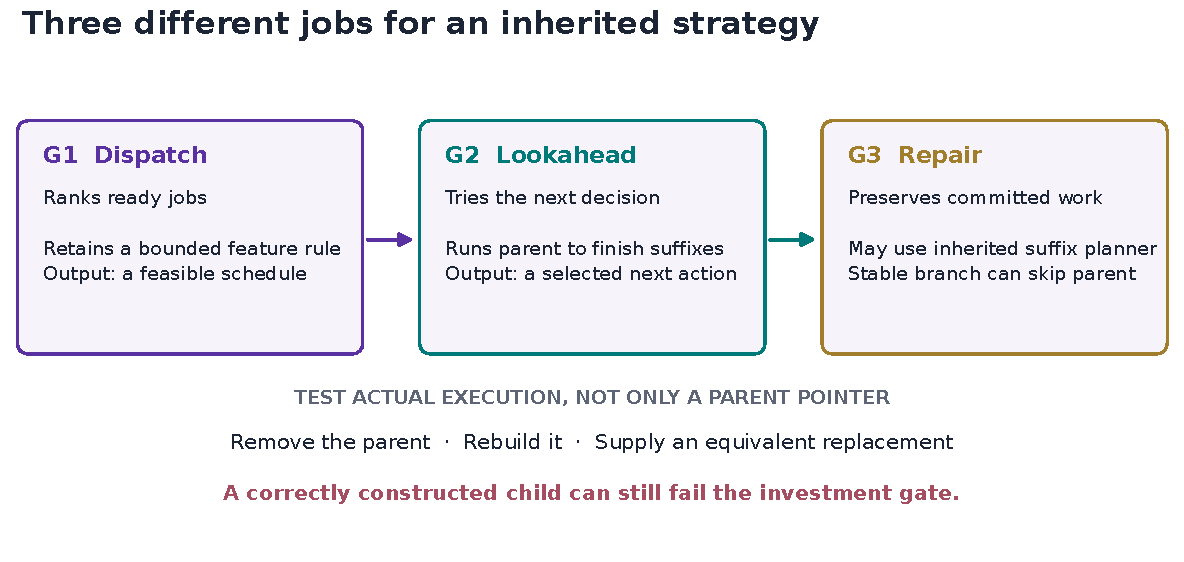
\includegraphics[width=\linewidth]{figures/generation-lineage.pdf}
\caption{The intended constructive dependency changes the method's contract. The diagnostic interventions distinguish a real inherited dependency from the economic decision to retain its child. Exact executed outcomes follow in the results.}\label{fig:lineage}
\end{figure}

\subsection{Bound discovery, maintenance and forgetting}

The controller searches only at registered opportunities, under an explicit debit limit, using a small new training batch and a disjoint qualification batch. It does not rescan the entire growing history after every job. A denied investment leaves the competent incumbent available. A stale dependency invalidates applicability; lack of useful remaining work produces defer or wait; an exhausted budget, deadline or authority scope produces stop or refusal. The archive records unsuccessful proposals without allowing their historical verdicts to become current admission.

Source inspection, AST validation, candidate execution, current checking, retention decisions and history work all have costs. The measured computational tariff is disclosed in the frozen protocol. It is a modeling instrument rather than a count of all physical machine instructions. Wall time, CPU time, stored bytes and intervention counts provide complementary views. Unmeasured authoring effort and human attention remain unknown; they are never silently entered as zero.
